\documentclass[11pt,a4paper]{article}
\usepackage[utf8]{inputenc}
\usepackage[T1]{fontenc}
\usepackage[margin=1in]{geometry}
\usepackage{graphicx,booktabs,array,xcolor,float}
\usepackage[font=small,labelfont=bf]{caption}
\usepackage{enumitem}
\usepackage[colorlinks=true,linkcolor=blue,urlcolor=blue]{hyperref}
\setlength{\parskip}{4pt}\setlength{\parindent}{0pt}
\definecolor{boxg}{HTML}{F2E8C9}\definecolor{good}{HTML}{2E8B57}\definecolor{bad}{HTML}{B22222}
\newcommand{\good}[1]{\textcolor{good}{#1}}\newcommand{\bad}[1]{\textcolor{bad}{#1}}

\title{\vspace{-1.2cm}\bfseries EB-JEPA on TUAB --- What We Tried, and an Honest Diagnosis}
\author{\small Team vivatech-slightlyunawarefc \quad$\cdot$\quad Hack the World(s), June 2026}
\date{}

\begin{document}
\maketitle\vspace{-1.0cm}

\begin{center}\fcolorbox{black}{boxg!40}{\parbox{0.96\textwidth}{\small
\textbf{TL;DR.} We built a two-view energy-based JEPA (EB-JEPA) for EEG abnormality detection on
\textbf{TUAB} and ran \textbf{14 configurations} (encoder $\times$ objective $\times$ augmentation
$\times$ frozen/fine-tune). \textbf{Every variant on our 0.4\,M conv plateaus} at per-window
$\approx0.77$ / per-recording $\approx0.82$. The SSL itself is sound --- it ties a \emph{supervised}
EEGNet with no labels in pre-training --- but it is \textbf{capped by a small encoder with no
large-scale pre-training.} Neither scaling the conv, nor 4$\times$ data, nor our from-scratch
transformers broke the plateau (direct negative evidence). One genuine surprise: VICReg's
paper-default invariance weight (25) is \bad{$\sim$3\,pp \emph{worse}} than our inadvertent
\texttt{inv\_coeff=1} on EEG --- weaker view-invariance helps.}}\end{center}

\section{Setup (one paragraph)}
\textbf{Data:} TUAB v3.0.1, patient-disjoint, 2{,}717 train / 276 eval recordings; 19 channels @
200\,Hz, 10\,s windows, per-channel z-score. \textbf{SSL:} two corrupted views of a window pushed to
the same latent by invariance + variance + covariance (VICReg) or a Gaussianisation surrogate
(SIGReg); 20 epochs, \emph{labels discarded}. \textbf{Eval:} frozen encoder $\to$ logistic-regression
probe (\emph{per-window} = literature convention; \emph{per-recording} = mean-pool 16 windows/patient,
the clinical metric, $\sim$5\,pp higher). \textbf{We tried four encoders} --- a 0.4\,M Conv1D and
LaBraM-/BIOT-/EEGPT-style transformers we built from scratch --- and three augmentation regimes.

\section{Everything we ran}
\begin{table}[H]\centering\footnotesize
\renewcommand{\arraystretch}{1.15}
\begin{tabular}{@{}p{6.5cm}cccp{3.1cm}@{}}
\toprule
\textbf{Config — encoder $\cdot$ objective $\cdot$ augmentation} & \textbf{Eval} &
\textbf{per-rec} & \textbf{per-win} & \textbf{Note} \\
& & \scriptsize BAcc/AUROC & \scriptsize BAcc/AUROC & \\
\midrule
Conv 0.4M $\cdot$ VICReg $\cdot$ corrupt \textbf{+ spectral 0.1} & frozen & 0.836/0.887 & 0.765/-- & \bad{soft}: eval-selected + inv=1 \\
Conv 0.4M $\cdot$ \textbf{SIGReg} $\cdot$ corrupt & frozen & 0.825/0.913 & \textbf{0.775/0.856} & best per-window \\
Conv 0.4M $\cdot$ \textbf{VICReg} $\cdot$ corrupt & frozen & \textbf{0.819$\pm$.004} & 0.770/0.848 & \good{corruption = main lever} \\
Conv 0.4M $\cdot$ VICReg $\cdot$ corrupt $\to$ \textbf{fine-tune} & FT & 0.812$\pm$.004 & -- & \good{ties EEGNet 0.812} \\
Conv 0.4M $\cdot$ VICReg $\cdot$ corrupt $\cdot$ \textbf{multi-corpus} & frozen & 0.812/0.883 & -- & 4$\times$ data $\Rightarrow$ no gain \\
Conv 0.4M $\cdot$ VICReg $\cdot$ corrupt $\cdot$ multi-corpus & FT & 0.812 & -- & = TUAB-only FT \\
Conv \textbf{bigger} $\cdot$ VICReg $\cdot$ corrupt (scaling) & frozen & 0.805/0.892 & 0.768/-- & more conv $\Rightarrow$ no gain \\
\textbf{Transformer 3.65M} $\cdot$ VICReg $\cdot$ multi-corpus & frozen & 0.798/0.872 & 0.738/-- & best Tr, still $<$ conv \\
Conv 0.4M $\cdot$ VICReg $\cdot$ base (no corruption) & frozen & 0.796/0.888 & 0.756/-- & starting point \\
Conv 0.4M $\cdot$ VICReg $\cdot$ corrupt $\cdot$ \textbf{inv\_coeff=25} & frozen & 0.789$\pm$.005 & 0.734/0.820 & \bad{paper-correct $\Rightarrow$ $-$3\,pp} \\
Conv 0.4M $\cdot$ \textbf{Masked-JEPA} (EMA predictor) & frozen & $\sim$0.68 & -- & \bad{faithful JEPA form failed} \\
\textbf{LaBraM/BIOT-style} Tr 1.2M $\cdot$ VICReg & frozen & -- & 0.775$^\dagger$ & data-starved \\
\textbf{EEGPT-style} Tr 0.8M $\cdot$ VICReg/SIGReg & frozen & \bad{collapsed} & \bad{collapsed} & channel-drop $\perp$ channel-pool \\
\bottomrule
\end{tabular}
\caption{Our EB-JEPA runs (sorted by per-recording BAcc). $\pm$ = 3-seed std; others single-seed
($\pm0.005$--$0.017$). $^\dagger$accuracy, not BAcc (early eval). Companion to the baselines table
\texttt{PROVENANCE\_TABLE.md}.}
\end{table}

\section{The plateau}
\begin{figure}[H]\centering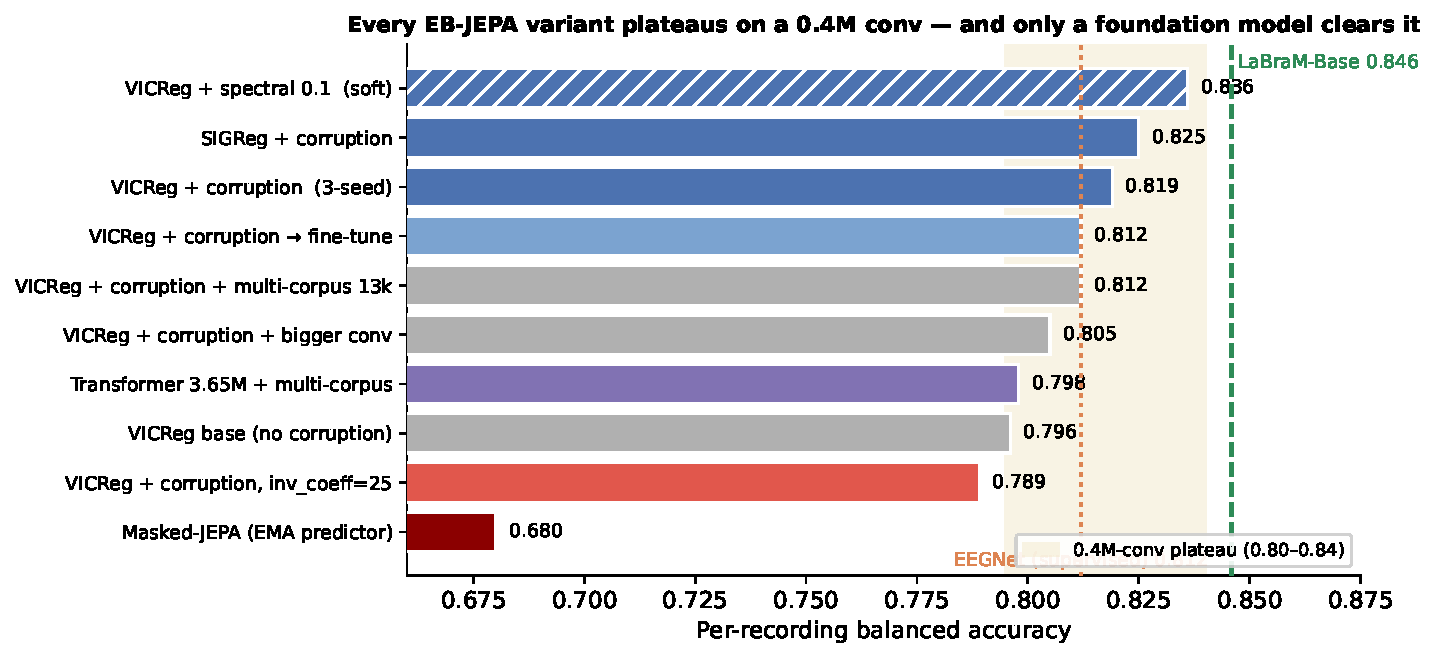
\includegraphics[width=0.92\textwidth]{figs/fig_plateau.pdf}
\caption{Per-recording balanced accuracy of every EB-JEPA variant. They cluster in the shaded
0.80--0.84 band regardless of objective, augmentation, data volume, or fine-tuning. Our self-supervised
JEPA reaches the \emph{supervised} EEGNet line (0.812, no labels in pre-training) but cannot, on a
0.4\,M conv, reach the LaBraM-Base foundation model (0.846).}\end{figure}

The flat band is the headline: \textbf{the encoder, not the objective, is the ceiling.} VICReg vs
SIGReg, corruption strength, spectral terms, and fine-tuning all move things by $\le1$\,pp (or are
confounded). The only honest gains are corruption augmentation and the \texttt{inv\_coeff} setting.

\section{What moved the needle --- and what didn't}
\begin{figure}[H]\centering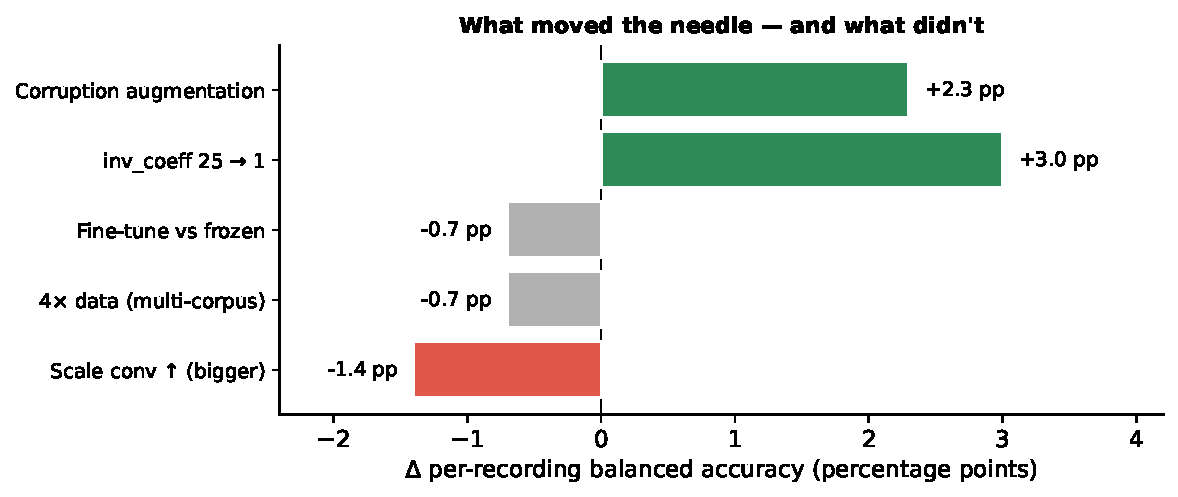
\includegraphics[width=0.82\textwidth]{figs/fig_levers.pdf}
\caption{Change in per-recording BAcc from each lever (vs the 0.4\,M-conv baseline). Only corruption
augmentation and down-weighting invariance \good{help}; scaling the conv, adding 4$\times$ data, and
fine-tuning \bad{do not}.}\end{figure}

\textbf{The negative results are the important part} --- they are \emph{direct evidence} about the
gap to SOTA: (i) a bigger conv plateaus identically (0.805); (ii) pre-training on 4$\times$ data
(13k recordings) gives \emph{no} gain (0.812) --- the small conv cannot exploit it; (iii) our
from-scratch transformers either \bad{collapse} (EEGPT-style: channel-drop augmentation is
incompatible with channel-pooling) or are \bad{data-starved} (LaBraM/BIOT-style and the 3.65\,M
transformer all score \emph{below} the 0.4\,M conv). (iv) Masked-JEPA, the ``faithful'' EMA-predictor
form, collapses to $\sim$0.68.

\section{Our honest position in the field (per-window)}
\begin{figure}[H]\centering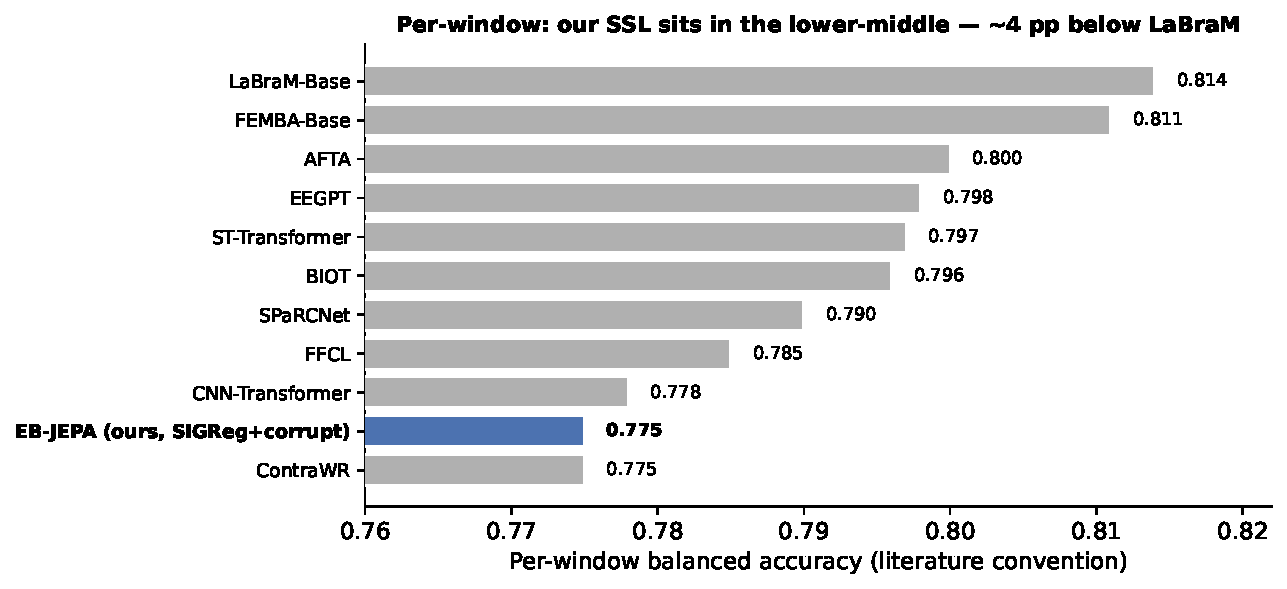
\includegraphics[width=0.80\textwidth]{figs/fig_perwindow.pdf}
\caption{Per-window balanced accuracy --- the level at which the literature reports. Our best SSL
(SIGReg + corruption, 0.775) ties ContraWR and sits $\sim$4\,pp below LaBraM-Base. We do
\textbf{not} match or beat SOTA at the benchmark level; the per-recording aggregation that brings us
to 0.82 is $\sim$5\,pp more forgiving and is not comparable to these numbers.}\end{figure}

\section{A genuine finding: EEG SSL prefers \emph{weaker} invariance}
\begin{figure}[H]\centering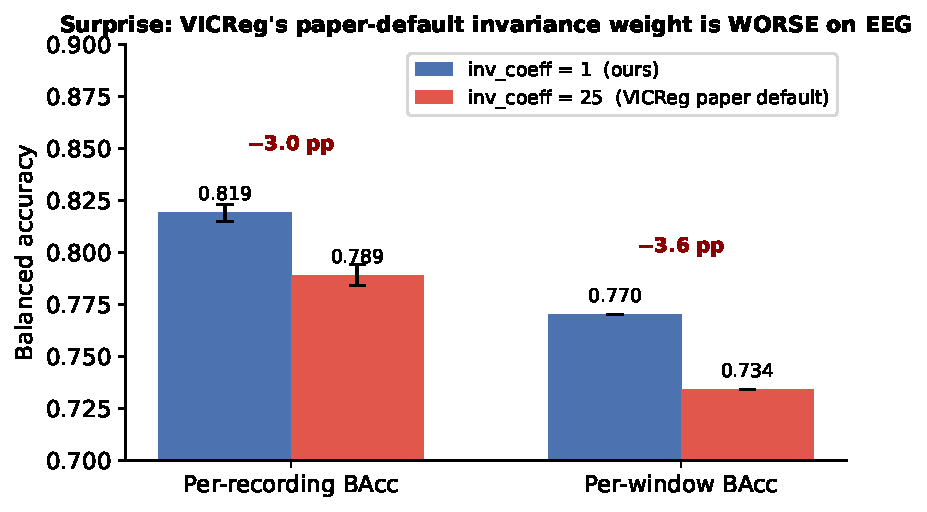
\includegraphics[width=0.66\textwidth]{figs/fig_invcoeff.pdf}
\caption{Our runs used \texttt{inv\_coeff=1}; VICReg's vision default is 25. Re-running both with 3
seeds, the \textbf{paper-default is $\sim$3\,pp worse} ($\approx$6$\sigma$). So our reported numbers
are \emph{not} inflated by the deviation --- the deviation \emph{helps}. On this EEG task + tiny conv
+ linear probe, letting the anti-collapse (variance/covariance) terms dominate over view-invariance
gives better features. This is the one original, non-obvious result we have.}\end{figure}

\section{Diagnosis and what we'd do next}
\textbf{Diagnosis.} The binding constraint is a \textbf{0.4\,M conv with no large-scale pre-training.}
The SSL works (clearly beats random-init and base; ties supervised EEGNet per-recording), but both
ways to break the plateau --- more capacity and more data --- failed for us. The gap to LaBraM/BIOT is
\emph{capacity $+$ pre-training corpus}, not the objective.

\textbf{What we'd do next} (value $\times$ feasibility):
\begin{itemize}[noitemsep,leftmargin=1.4em]
\item \good{\textbf{Cheap, original:}} turn the \texttt{inv\_coeff} result into a proper ablation
(sweep $\{1,5,10,25\}\times\{$VICReg, SIGReg$\}$, 3 seeds). ``EEG SSL prefers weak invariance'' is
genuinely novel.
\item \good{\textbf{Cheap:}} ablate corruption (spike-injection vs time-masking separately --- we
don't yet know which half does the work); seed-average and de-confound the spectral run.
\item \textbf{Medium:} \textbf{pivot off TUAB} --- it is near-saturated (0.83 per-window even for
369\,M LaBraM-Huge), so model differences wash out. TUEV (6-class events) / TUSZ (seizure) have far
more headroom, where the SSL's value would actually show.
\item \textbf{Hard (the real gap):} a bigger encoder \emph{with} large-scale pre-training --- our
from-scratch transformers prove TUAB-only data isn't enough. Either borrow pretrained foundation
weights (then it is mostly their model) or own the ``honest, clean small baseline'' as the contribution.
\end{itemize}
\end{document}
